\documentclass{IEEE_lsens}

\usepackage{textcomp}
\usepackage[noadjust]{cite}
\usepackage[T1]{fontenc}
\usepackage{amsmath}
\interdisplaylinepenalty=2500
\usepackage[cmintegrals]{newtxmath}
\usepackage{bm}
\usepackage{array}
\usepackage{algorithmic}
\usepackage{url}
\usepackage{graphicx}
\graphicspath{{./}{paper_assets/}}
\usepackage{tikz}
\usetikzlibrary{arrows.meta, positioning, calc, shapes.geometric}

\providecommand{\hypersetup}[1]{\relax}
\providecommand{\texorpdfstring}[2]{#1}

\hyphenation{op-tical net-works semi-conduc-tor}

% ===================================================================
% NOTE (remove before submission):
%  * IEEE Sensors Letters has a HARD 4-page limit (references included).
%  * This draft keeps ONE table (on-device timing, all measured) and three
%    self-contained TikZ figures (pipeline, STD machine, SR gate) that
%    render with no image files. All placeholder/TBD tables and figures
%    were removed; only measured or clearly-defined content remains.
%  * The reference list is ~17 entries (not 35+) to respect the page cap;
%    re-check final venues/pages on IEEE Xplore before submission.
%  * DOUBLE-BLIND: author block, affiliation, funding/acknowledgment, and
%    identifying code/data URLs withheld; no self-identifying citations.
% ===================================================================

\begin{document}

\markboth{IEEE Sensors Letters}{0000000}

\IEEELSENSarticlesubject{Sensor Applications}

\title{An On-Device Eye-Blink Sensing Pipeline for the Raspberry~Pi~5:
Per-Subject EAR Calibration and a Quality-Conditioned Super-Resolution Gate}

\author{\IEEEauthorblockN{Anonymous Author(s)}%
\IEEEauthorblockA{Affiliation withheld for double-blind review}%
\thanks{Corresponding author: withheld for review.}%
\thanks{Associate Editor: [TBD].}%
\thanks{This work is submitted for double-blind review; funding and
acknowledgments are withheld. Code and evaluation data are available at an
anonymized repository (link withheld for review).}%
\thanks{Digital Object Identifier 10.1109/LSENS.XXXX.XXXXXXX}}
\IEEELSENSmanuscriptreceived{Manuscript received [Month] [Day], [Year];
accepted [Month] [Day], [Year]. Date of publication [Month] [Day], [Year];
date of current version [Month] [Day], [Year].}

\IEEEtitleabstractindextext{%
\begin{abstract}
This letter presents an on-device eye-blink sensing pipeline in which a
single RGB camera is turned into a robust real-time blink counter on a
Raspberry~Pi~5. Eye-corner landmarks from MediaPipe FaceLandmarker drive an
Eye Aspect Ratio (EAR) signal, a brief per-subject calibration stage replaces
subject-independent fixed thresholds with personalized open/closed statistics,
and a four-state (Open--Closing--Closed--Reopening) machine with hysteresis
counts a blink only on a completed cycle. To sustain landmark quality when the
ocular region is small, we further propose a quality-conditioned
super-resolution (SR) gate that upsamples only the face region-of-interest, and
only when the measured eye width falls below a pixel threshold. On-device
measurements indicate a sustained throughput of about 25~fps with a mean
FaceLandmarker latency of 24.2~ms per frame (95th percentile 26.3~ms), and the
baseline detector remains lossless under downscaling up to $6\times$ on a
representative distant clip. A preliminary on-device study further indicates
that the conditional SR gate is worthwhile only within a narrow low-quality
band, because the baseline is already robust wherever ocular information
survives.
\end{abstract}
\begin{IEEEkeywords}
Eye-blink sensing, eye aspect ratio, edge computing, Raspberry Pi,
per-subject calibration, super-resolution, landmark localization,
real-time vision sensing.
\end{IEEEkeywords}}

\maketitle

\section{Introduction}
\IEEEPARstart{V}{ision}-based eye-blink sensing---estimating when and how often
a person blinks from ordinary RGB frames---underpins applications such as
eye-strain and fatigue monitoring, attention estimation, and human--computer
interaction. Deploying such sensing \emph{on-device}, at the edge, is
attractive because it avoids streaming video off the camera and enables
low-latency, privacy-preserving operation. Realizing this on a low-power
single-board computer, however, exposes three coupled difficulties that
motivate this work.

First, many edge-oriented systems deploy general-purpose object-detection
backbones and operate in a \emph{batch} fashion, accumulating several seconds
of video before producing a blink-rate estimate, which limits per-frame
responsiveness on constrained hardware~\cite{carcellar2024,reddy2019}. Second,
blink decisions typically rely on \emph{fixed, subject-independent} EAR
thresholds~\cite{soukupova2016}, ignoring inter-subject variability in eyelid
geometry, palpebral aperture, and eyewear, which inflates false positives for
users whose resting EAR differs from the assumed value~\cite{drowsy2025}. Third,
when the ocular region is small or of low quality---a distant or low-resolution
subject---landmark localization degrades~\cite{bulat2018}; enhancing the
\emph{entire} frame with SR at every timestep can mitigate this but imposes a
computational cost that is difficult to sustain in real time at the
edge~\cite{dong2016}. Notably, sequential ``enhance-then-detect'' pipelines are
not guaranteed to help and can even hurt when the enhanced image departs from
the detector's training distribution, so any such enhancement must be validated
rather than assumed beneficial. This letter deliberately separates what is
\emph{measured on-device} from what is \emph{still under evaluation}.

This letter presents a lightweight, real-time blink-sensing pipeline for the
Raspberry~Pi~5 that couples per-subject calibration with a quality-conditioned
SR gate. Rather than a fixed threshold, the system estimates subject-specific
open/closed EAR statistics during a brief calibration stage and injects the
resulting personalized thresholds into a four-state machine with hysteresis.
Rather than enhancing every frame, a conditional gate triggers a lightweight SR
model (e.g., FSRCNN-small or ESPCN~\cite{dong2016,shi2016}) only on the
face ROI, and only when the eye width in pixels falls below a predefined
criterion. Because EAR is a scale-invariant ratio, the value of SR is not to
``enlarge'' the signal but to stabilize where the landmarks are localized under
low quality---so we treat the gate as a hypothesis to be tested on-device, not a
settled result. Our contributions are threefold:
\begin{itemize}
\item a \emph{per-subject EAR calibration} stage that replaces
subject-independent fixed thresholds with personalized open/closed statistics
and hysteresis bands, injected into a four-state (Open--Closing--Closed--%
Reopening) machine that counts a blink only on a completed cycle;
\item a \emph{quality-conditioned, eye-pixel-driven SR gate} that applies a
lightweight face-ROI two-pass super-resolution only when the measured eye width
drops below a hysteretic pixel threshold, confining the added computation to the
frames that plausibly need it;
\item an \emph{on-device characterization} on the Raspberry~Pi~5 that reports
sustained throughput and landmark latency, quantifies baseline robustness to
image downscaling, and---through a preliminary go/no-go study---delineates the
narrow operating band in which the conditional SR gate is worthwhile.
\end{itemize}

\section{Related Work}
\emph{EAR-based blink detection.} Soukupov\'a and \v{C}ech~\cite{soukupova2016}
defined the EAR from six eye landmarks and established a basis for real-time
blink detection; the metric is widely reused but its fixed global threshold does
not capture individual differences. Fogelton and Bene\v{s}ov\'a~\cite{fogelton2016}
proposed a motion-vector--based blink detector and released the Eyeblink8
sequence, which, together with the TalkingFace video~\cite{talkingface}, remains
a standard evaluation reference. Kwon \textit{et al.}~\cite{kwon2013} characterized blink kinematics
(closing faster than reopening, $\approx$0.5\,s duration), which grounds the use
of an ordered state machine rather than per-frame decisions.

\emph{Robust and in-the-wild detection.} Zeng \textit{et al.}~\cite{zeng2023}
proposed a one-stage instance-level detector with a large in-the-wild dataset,
and RT-BENE~\cite{cortacero2019} provides a real-time blink-estimation
benchmark; both, however, assume GPU-class compute and are used here only as
non-edge reference points.

\emph{Personalization and quality enhancement.} Personalized EAR/MAR thresholds
have been shown to reduce inter-subject error in drowsiness
detection~\cite{drowsy2025}, and a low-light pipeline based on
Zero-DCE~\cite{guo2020} couples image enhancement with joint face/landmark
detection and EAR for nighttime fatigue~\cite{lowlight2025}; both target
non-edge, always-on enhancement and do not gate enhancement by ocular pixel
quality. In the super-resolution literature, FSRCNN~\cite{dong2016} and
ESPCN~\cite{shi2016} are lightweight enough for edge use, while
Super-FAN~\cite{bulat2018} jointly localizes landmarks and super-resolves faces. Our closest edge
baseline is a Raspberry~Pi blink-rate eye-strain system~\cite{carcellar2024}
that uses a heavy detector with batch processing and no personalization or
conditional enhancement. Relative to these, the proposed pipeline is
distinguished by combining per-subject personalization, cycle-based counting,
and quality-conditioned enhancement in a single real-time on-device loop.

\section{Method}
\begin{figure}[!t]
\centering
\resizebox{\columnwidth}{!}{%
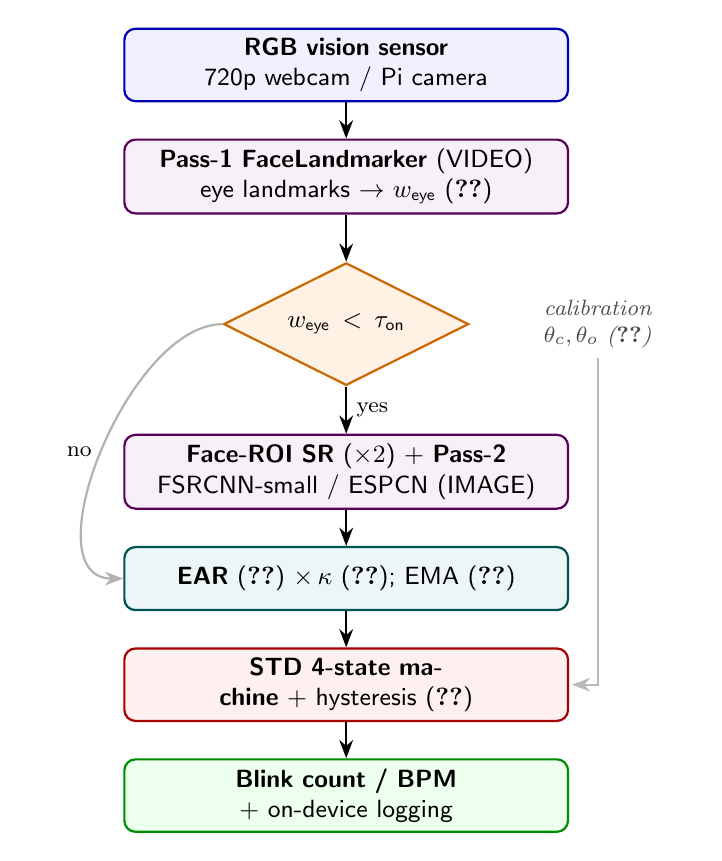
\begin{tikzpicture}[
    font=\sffamily\small, >=Stealth, node distance=4.6mm,
    sensor/.style={rectangle, rounded corners, draw=blue!70!black,   thick, fill=blue!6,   text width=5.4cm, align=center, minimum height=0.8cm},
    proc/.style  ={rectangle, rounded corners, draw=violet!70!black, thick, fill=violet!6, text width=5.4cm, align=center, minimum height=0.8cm},
    gate/.style  ={diamond, aspect=2, draw=orange!80!black, thick, fill=orange!10, align=center, inner sep=1pt, text width=2.4cm},
    feat/.style  ={rectangle, rounded corners, draw=teal!65!black,   thick, fill=teal!7,   text width=5.4cm, align=center, minimum height=0.8cm},
    sm/.style    ={rectangle, rounded corners, draw=red!65!black,    thick, fill=red!6,    text width=5.4cm, align=center, minimum height=0.8cm},
    result/.style={rectangle, rounded corners, draw=green!55!black,  thick, fill=green!7,  text width=5.4cm, align=center, minimum height=0.8cm},
    note/.style  ={draw=none, fill=none, text=gray!60!black, font=\footnotesize\itshape, text width=2.2cm, align=center},
]
\node[sensor] (cam) {\textbf{RGB vision sensor}\\ 720p webcam / Pi camera};
\node[proc, below=of cam]  (mp1)  {\textbf{Pass-1 FaceLandmarker} (VIDEO)\\ eye landmarks $\rightarrow$ $w_{\text{eye}}$ (\ref{eq_weye})};
\node[gate, below=6mm of mp1] (g)  {$w_{\text{eye}}<\tau_{\text{on}}$};
\node[proc, below=6mm of g] (sr)  {\textbf{Face-ROI SR} ($\times 2$) + \textbf{Pass-2}\\ FSRCNN-small / ESPCN (IMAGE)};
\node[feat, below=of sr]   (feat) {\textbf{EAR} (\ref{eq_ear}) $\times\,\kappa$ (\ref{eq_kappa}); EMA (\ref{eq_ema})};
\node[sm,   below=of feat] (sm)   {\textbf{STD 4-state machine} + hysteresis (\ref{eq_thresh})};
\node[result, below=of sm] (res)  {\textbf{Blink count / BPM} + on-device logging};
\node[note, right=4mm of g] (cal) {calibration\\ $\theta_c,\theta_o$ (\ref{eq_calib})};
\draw[->,thick] (cam)--(mp1);
\draw[->,thick] (mp1)--(g);
\draw[->,thick] (g)-- node[right,font=\footnotesize]{yes} (sr);
\draw[->,thick] (sr)--(feat);
\draw[->,thick] (feat)--(sm);
\draw[->,thick] (sm)--(res);
\draw[->,thick,draw=gray!60] (g.west) .. controls +(-1.2,0) and +(-1.2,0) .. node[left,font=\footnotesize]{no} (feat.west);
\draw[->,thick,draw=gray!55, shorten >=1pt] (cal.south) |- (sm.east);
\end{tikzpicture}}
\caption{Overall on-device pipeline. A single RGB frame is localized by a first
FaceLandmarker pass to obtain the eye width $w_{\text{eye}}$; a quality gate
routes only low-quality frames through a face-ROI super-resolution and a second
landmark pass, after which the EAR feeds a per-subject-calibrated four-state
(Open--Closing--Closed--Reopening) machine that emits blink counts and BPM. All
stages run in a single real-time loop on the Raspberry~Pi~5.}
\label{fig_arch}
\end{figure}
The pipeline (Figs.~\ref{fig_arch} and~\ref{alg_pipeline}) processes each
frame through landmark extraction, a quality gate, EAR computation, and a
cycle-based state machine, all within one real-time loop.

\subsection{Per-Subject EAR Calibration}
Facial landmarks are extracted with MediaPipe
FaceLandmarker~\cite{lugaresi2019}, whose detector builds on
BlazeFace~\cite{bazarevsky2019}. For each eye, the EAR is computed from six
landmarks $\bm{p}_1,\dots,\bm{p}_6$,
\begin{equation}
\mathrm{EAR}=\frac{\lVert \bm{p}_2-\bm{p}_6\rVert+\lVert \bm{p}_3-\bm{p}_5\rVert}
{2\,\lVert \bm{p}_1-\bm{p}_4\rVert},
\label{eq_ear}
\end{equation}
and the per-frame value is the mean of the two eyes, multiplied by a head-pose
correction factor $\kappa$ that compensates for foreshortening at oblique
angles,
\begin{equation}
\kappa = 1 + \alpha\left(1 - \min\!\left(\frac{d}{d_0},\,1\right)\right),
\label{eq_kappa}
\end{equation}
where $d$ is the normalized inter-ocular distance, $d_0$ a frontal reference,
and $\alpha$ a small maximum boost. The raw signal is smoothed by an
exponential moving average with factor $\gamma$,
\begin{equation}
\widetilde{\mathrm{EAR}}_t=\gamma\,\mathrm{EAR}_t+(1-\gamma)\,\widetilde{\mathrm{EAR}}_{t-1}.
\label{eq_ema}
\end{equation}

During calibration the system records open-eye frames (eyes held open) and
closed-eye frames (eyes held shut) and estimates the personalized baseline as a
high percentile $q$ of the open-eye EAR distribution,
$\mathrm{EAR}_{\text{open}}=\mathrm{Perc}_q\{\mathrm{EAR}_i^{\text{open}}\}$, and
$\mathrm{EAR}_{\text{closed}}=\mathrm{mean}\{\mathrm{EAR}_i^{\text{closed}}\}$.
Two hysteresis thresholds are then set relative to the per-subject baseline,
\begin{equation}
\theta_c=\beta_c\,\mathrm{EAR}_{\text{open}},\qquad
\theta_o=\beta_o\,\mathrm{EAR}_{\text{open}},\qquad \beta_c<\beta_o,
\label{eq_thresh}
\end{equation}
with $\theta_c$ the closing threshold and $\theta_o$ the reopening threshold;
the gap $[\theta_c,\theta_o]$ suppresses state chatter from EAR jitter. Both
thresholds are periodically refreshed over a sliding window to track slow
illumination drift. Compactly, calibration produces the personalized parameter
set
\begin{equation}
\Theta=\big(\mathrm{EAR}_{\text{open}},\,\mathrm{EAR}_{\text{closed}},\,\theta_c,\,\theta_o\big).
\label{eq_calib}
\end{equation}

\subsection{Four-State Blink Machine (STD)}
\begin{figure}[!t]
\centering
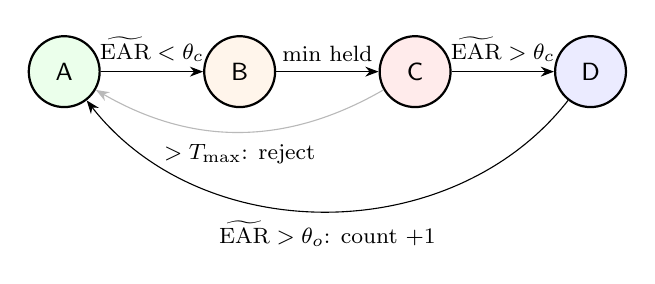
\begin{tikzpicture}[font=\sffamily\small, >=Stealth, node distance=13mm,
   st/.style={circle, draw, thick, minimum size=9mm, inner sep=1pt}]
\node[st, fill=green!8]  (A) {A};
\node[st, fill=orange!8, right=of A] (B) {B};
\node[st, fill=red!8,    right=of B] (C) {C};
\node[st, fill=blue!8,   right=of C] (D) {D};
\draw[->] (A) -- node[above,font=\footnotesize]{$\widetilde{\mathrm{EAR}}<\theta_c$} (B);
\draw[->] (B) -- node[above,font=\footnotesize]{min held} (C);
\draw[->] (C) -- node[above,font=\footnotesize]{$\widetilde{\mathrm{EAR}}>\theta_c$} (D);
\draw[->,gray!55] (C) to[bend left=30] node[below=1pt,font=\footnotesize,text=black,pos=0.5]{$>T_{\max}$: reject} (A);
\draw[->] (D) to[bend left=52] node[below,font=\footnotesize]{$\widetilde{\mathrm{EAR}}>\theta_o$: count $+1$} (A);
\end{tikzpicture}
\caption{Four-state blink machine:
A (Open) $\rightarrow$ B (Closing) $\rightarrow$ C (Closed) $\rightarrow$
D (Reopening) $\rightarrow$ A. A blink is counted only on a completed cycle,
which rejects half-blinks and per-frame noise. The B$\rightarrow$C transition
(``min held'') requires the EAR minimum to persist for a minimum number of
frames, and a closed interval longer than $T_{\max}$ is rejected as a
drowsy/downward-gaze episode rather than counted.}
\label{fig_std}
\end{figure}
The blink decision is made by a four-state state-transition detector (STD).
From the instant $\widetilde{\mathrm{EAR}}$ falls below $\theta_c$ until it
recovers above $\theta_o$, a blink is tracked by the ordered STD machine of
Fig.~\ref{fig_std}. A blink is counted only when the full A$\rightarrow$B%
$\rightarrow$C$\rightarrow$D$\rightarrow$A cycle completes, so a single
prolonged closure is not miscounted as many frame-level events, and a closed
interval exceeding $T_{\max}$ is rejected as drowsiness rather than a blink.

\subsection{Quality-Conditioned Super-Resolution Gate}
\begin{figure}[!t]
\centering
\resizebox{\columnwidth}{!}{%
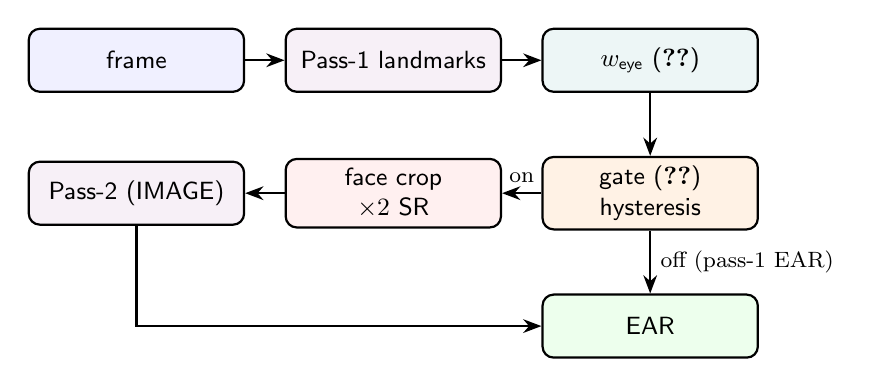
\begin{tikzpicture}[font=\sffamily\small, >=Stealth, node distance=5mm,
    b/.style={rectangle, rounded corners, draw, thick, text width=2.5cm, align=center, minimum height=0.8cm}]
\node[b, fill=blue!6]   (in)  {frame};
\node[b, fill=violet!6, right=of in] (p1) {Pass-1 landmarks};
\node[b, fill=teal!7, right=of p1]   (w)  {$w_{\text{eye}}$ (\ref{eq_weye})};
\node[b, fill=orange!10, below=8mm of w] (dec) {gate (\ref{eq_gate})\\hysteresis};
\node[b, fill=red!6, left=of dec]    (crop){face crop\\ $\times 2$ SR};
\node[b, fill=violet!6, left=of crop](p2)  {Pass-2 (IMAGE)};
\node[b, fill=green!7, below=8mm of dec] (ear) {EAR};
\draw[->,thick](in)--(p1); \draw[->,thick](p1)--(w); \draw[->,thick](w)--(dec);
\draw[->,thick](dec)-- node[above,font=\footnotesize]{on}(crop);
\draw[->,thick](crop)--(p2);
\draw[->,thick](p2) |- (ear);
\draw[->,thick](dec)-- node[right,font=\footnotesize]{off (pass-1 EAR)}(ear);
\end{tikzpicture}}
\caption{Face-ROI two-pass SR gate (detail of the gated branch in
Fig.~\ref{fig_arch}). A first pass yields $w_{\text{eye}}$; when the gate fires,
the face crop is upsampled $\times2$ and re-localized by a second (stateless
IMAGE-mode) pass. As EAR is scale-invariant, EAR is read directly in the
upsampled frame with no inverse coordinate mapping.}
\label{fig_srgate}
\end{figure}
Because the FaceLandmarker consumes a whole face rather than an isolated eye
patch, SR is applied to the \emph{face} ROI in a two-pass arrangement
(Fig.~\ref{fig_srgate}). The gate signal is the per-frame eye width in pixels,
\begin{equation}
w_{\text{eye}}=\tfrac{1}{2}\big(\lVert \bm{p}_1^{L}-\bm{p}_4^{L}\rVert
+\lVert \bm{p}_1^{R}-\bm{p}_4^{R}\rVert\big)\cdot W,
\label{eq_weye}
\end{equation}
where $\bm{p}_1,\bm{p}_4$ are the normalized eye-corner landmarks and $W$ the
frame width. To avoid chattering, the gate uses hysteresis with an on-threshold
$\tau_{\text{on}}$ and a larger off-threshold $\tau_{\text{off}}$,
\begin{equation}
g_t=\begin{cases}
1, & w_{\text{eye}}<\tau_{\text{on}}\\[2pt]
0, & w_{\text{eye}}\ge \tau_{\text{off}}\\[2pt]
g_{t-1}, & \text{otherwise,}
\end{cases}
\label{eq_gate}
\end{equation}
with $\tau_{\text{on}}<\tau_{\text{off}}$. When $g_t=1$, the face crop (with
margin) is upsampled $\times2$ by a lightweight model (FSRCNN-small or ESPCN via
OpenCV \texttt{dnn\_superres}) and re-localized; otherwise the first-pass EAR is
used unchanged, preserving the real-time path. Because EAR is a ratio of
normalized coordinates, its \emph{value} is invariant to this rescaling, so any
benefit of SR arises solely from more stable landmark localization under low
quality---a hypothesis we test directly on-device (Sec.~\ref{sec_srgo}). In our
configuration, the open baseline uses the 80th percentile ($q$), the EMA factor
is $\gamma=0.5$, the gate thresholds are $\tau_{\text{on}}=24$~px and
$\tau_{\text{off}}=30$~px, and $T_{\max}=1.0$~s; the closing/reopening fractions
$\beta_c<\beta_o$ and the pose-boost $\alpha$ are fixed small constants.

\begin{figure}[!t]
\begin{algorithmic}[1]
\renewcommand{\algorithmicrequire}{\textbf{Input:}}
\renewcommand{\algorithmicensure}{\textbf{Output:}}
\REQUIRE RGB frame stream; calibrated $\Theta$ (\ref{eq_calib})
\ENSURE per-frame blink state; blink count / BPM
\STATE calibrate: set $\mathrm{EAR}_{\text{open}},\theta_c,\theta_o$ (\ref{eq_calib})
\FOR{each frame}
  \STATE pass-1 landmarks; compute $w_{\text{eye}}$ (\ref{eq_weye})
  \IF{$g_t=1$ (gate fires by hysteresis, \ref{eq_gate})}
     \STATE upsample face ROI $\times2$; pass-2 landmarks (IMAGE)
  \ENDIF
  \STATE EAR (\ref{eq_ear})$\times\kappa$ (\ref{eq_kappa}); EMA (\ref{eq_ema})
  \STATE update STD machine; on full cycle: count$+1$; update BPM
\ENDFOR
\end{algorithmic}
\caption{Pseudocode of the real-time on-device blink-sensing loop.}
\label{alg_pipeline}
\end{figure}

\section{Experiments}
\subsection{Setup}
The pipeline runs on a Raspberry~Pi~5 (aarch64) fed by an RGB webcam over an
MJPEG stream, using MediaPipe FaceLandmarker, OpenCV, and NumPy only.
On-device timing is measured with a per-frame profiler over more than 3000
frames; blink-count robustness is probed by synthetically downscaling a
self-captured distant clip with a known reference count prior to detection.

\subsection{On-Device Real-Time Feasibility}
\begin{table}[!t]
\caption{On-Device Timing and Throughput (Raspberry~Pi~5, Measured).}
\label{table_edge}
\centering
\renewcommand{\arraystretch}{1.25}
\begin{tabular*}{\columnwidth}{l@{\extracolsep{\fill}}c}
\hline\hline
Quantity & Value\\
\hline
FaceLandmarker latency, mean & 24.2~ms\\
FaceLandmarker latency, 95th percentile & 26.3~ms\\
Sustained pipeline throughput (no SR) & $\approx$25~fps\\
FaceLandmarker throughput ceiling & $\approx$41~fps\\
Face-ROI SR $\times2$ upsample (distant face) & $\approx$50~ms\\
Two-pass SR frame (SR $+$ second pass) & $\approx$100~ms ($\approx$10~fps)\\
\hline\hline
\end{tabular*}
\end{table}
Table~\ref{table_edge} summarizes on-device timing. The FaceLandmarker front end
dominates cost at a mean of 24.2~ms per frame (95th percentile 26.3~ms),
yielding a sustained pipeline throughput of about 25~fps. The gap between the
$\approx$41~fps landmark ceiling ($1/24.2$~ms) and the $\approx$25~fps
end-to-end rate is due to MJPEG stream decoding, frame capture, and per-frame
logging that surround the inference step; even so, a 24~fps operating point
leaves headroom of the order of 15~ms per frame. A face-ROI SR upsample
adds roughly 50~ms for a small (distant) face, and a full two-pass SR frame
reaches about 100~ms ($\approx$10~fps); this falls below a 15~fps floor, which
is precisely why SR is confined to gated frames rather than applied
continuously.

\subsection{Baseline Robustness to Downscaling}
To probe robustness, a self-captured distant clip with a reference count of
about 29 blinks was progressively downscaled before detection. The baseline
detector (SR off) recovered the reference count without loss up to $6\times$
downscaling, and only lost blinks at the extreme $8\times$ setting (27 detected),
where the ocular region becomes too small to localize reliably. In other words,
wherever ocular information survives, the personalized cycle-based baseline is
already accurate.

\subsection{Conditional SR Gate: Preliminary Go/No-Go}
\label{sec_srgo}
Because the baseline already succeeds wherever ocular information survives, the
gate contributes little. At normal scales it stays essentially inactive; at a
mild $2\times$ setting it fires on many frames yet leaves the count unchanged
(harmless but not helpful); and only at the extreme $8\times$ setting---where
EAR information is already lost---does it fire on nearly every frame, there
fabricating high-frequency detail that slightly \emph{degrades} the count
($27\!\rightarrow\!25$). These preliminary on-device results suggest that the
useful ``middle band'' for conditional SR is narrow in this pipeline, and they
operationalize the known risk that sequential enhance-then-detect can hurt. We
therefore report the conditional SR gate as a proposed and partially
characterized mechanism whose adoption is contingent on further evaluation,
rather than as a settled performance gain.

\subsection{Discussion and Limitations}
The measured results support two claims: the pipeline sustains real-time
operation ($\approx$25~fps) on the Raspberry~Pi~5, and the personalized,
cycle-based baseline is robust to substantial downscaling ($\le 6\times$). The
conditional SR gate is presented as a proposed mechanism whose on-device benefit
is not yet established: because EAR is scale-invariant and the baseline is
already robust, the gate's useful operating band appears narrow, and at extreme
degradation SR can hurt. The main limitations follow directly. The robustness
evidence comes from a single self-captured clip, so low-light conditions and
eyewear are not yet covered, and multi-subject calibration accuracy and
detection F1 against external annotations remain to be established. Future work
will add a bicubic-upsampling control to separate ``learned SR'' from ``mere
resampling'' and evaluate a low-light enhancement alternative~\cite{guo2020}.

\section{Conclusion}
This letter described an on-device eye-blink sensing pipeline for the
Raspberry~Pi~5 that combines per-subject EAR calibration, a hysteretic
four-state blink machine, and a quality-conditioned face-ROI super-resolution
gate. On-device measurements confirm real-time throughput ($\approx$25~fps) and
baseline robustness to downscaling up to $6\times$, while a preliminary go/no-go
study characterizes the narrow band in which the conditional SR gate is
warranted. Future work will extend the evaluation to multiple subjects and
low-light conditions and consider INT8 quantization~\cite{jacob2018} for tighter
edge budgets.

\begin{thebibliography}{20}

\bibitem{soukupova2016}
T.~Soukupov\'a and J.~\v{C}ech, ``Real-time eye blink detection using facial
landmarks,'' in \emph{Proc. 21st Comput. Vis. Winter Workshop (CVWW)}, 2016,
pp.~1--8.

\bibitem{fogelton2016}
A.~Fogelton and W.~Bene\v{s}ov\'a, ``Eye blink detection based on motion vectors
analysis,'' \emph{Comput. Vis. Image Understanding}, vol.~148, pp.~23--33, 2016.

\bibitem{talkingface}
``Talking face video,'' FGnet Project (IST-2000-26434), 2004. [Online].
Available: standard blink-annotated evaluation sequence.

\bibitem{kwon2013}
K.-A. Kwon \textit{et al.}, ``High-speed camera characterization of voluntary
eye blinking kinematics,'' \emph{J. R. Soc. Interface}, vol.~10, no.~85, 2013,
Art. no.~20130227.

\bibitem{zeng2023}
W.~Zeng \textit{et al.}, ``Real-time multi-person eyeblink detection in the wild
for untrimmed video,'' in \emph{Proc. IEEE/CVF Conf. Comput. Vis. Pattern
Recognit. (CVPR)}, 2023, pp.~13854--13863.

\bibitem{cortacero2019}
K.~Cortacero, T.~Fischer, and Y.~Demiris, ``RT-BENE: A dataset and baselines for
real-time blink estimation in natural environments,'' in \emph{Proc. IEEE/CVF
Int. Conf. Comput. Vis. Workshops (ICCVW)}, 2019, pp.~1159--1168.

\bibitem{carcellar2024}
R.~Carcellar, J.~Tychuaco, and N.~Yumang, ``Self-applicable eye strain detection
through the measurement of blink rate using Raspberry Pi,'' in \emph{Proc. IEEE
Int. Conf. Artif. Intell. Eng. Technol. (IICAIET)}, 2024.

\bibitem{reddy2019}
A.~P.~C. Reddy, B.~V.~H. Sandilya, and A.~Annis~Fathima, ``Detection of eye
strain through blink rate and sclera area using raspberry-pi,'' \emph{Imaging
Sci. J.}, vol.~67, no.~2, pp.~90--99, 2019.

\bibitem{drowsy2025}
G.~Ersoy, M.~A. Tatar, E.~Tonbul, and S.~K{\i}rb{\i}z, ``Improving driver
drowsiness detection via personalized EAR/MAR thresholds and CNN-based
classification,'' 2026, \emph{arXiv:2604.22479}.

\bibitem{lowlight2025}
Z.~Huang, J.~Huang, and J.~Huang, ``Nighttime driver fatigue detection based on
real-time joint face and facial landmarks detection,'' \emph{Modelling},
vol.~7, no.~2, 2026, Art. no.~60.

\bibitem{lugaresi2019}
C.~Lugaresi \textit{et al.}, ``MediaPipe: A framework for building perception
pipelines,'' 2019, \emph{arXiv:1906.08172}.

\bibitem{bazarevsky2019}
V.~Bazarevsky \textit{et al.}, ``BlazeFace: Sub-millisecond neural face detection
on mobile GPUs,'' 2019, \emph{arXiv:1907.05047}.

\bibitem{dong2016}
C.~Dong, C.~C. Loy, and X.~Tang, ``Accelerating the super-resolution
convolutional neural network,'' in \emph{Proc. Eur. Conf. Comput. Vis. (ECCV)},
2016, pp.~391--407.

\bibitem{shi2016}
W.~Shi \textit{et al.}, ``Real-time single image and video super-resolution
using an efficient sub-pixel convolutional neural network,'' in \emph{Proc.
IEEE Conf. Comput. Vis. Pattern Recognit. (CVPR)}, 2016, pp.~1874--1883.

\bibitem{bulat2018}
A.~Bulat and G.~Tzimiropoulos, ``Super-FAN: Integrated facial landmark
localization and super-resolution of real-world low resolution faces,'' in
\emph{Proc. IEEE Conf. Comput. Vis. Pattern Recognit. (CVPR)}, 2018,
pp.~109--117.

\bibitem{guo2020}
C.~Guo \textit{et al.}, ``Zero-reference deep curve estimation for low-light
image enhancement,'' in \emph{Proc. IEEE/CVF Conf. Comput. Vis. Pattern
Recognit. (CVPR)}, 2020, pp.~1780--1789.

\bibitem{jacob2018}
B.~Jacob \textit{et al.}, ``Quantization and training of neural networks for
efficient integer-arithmetic-only inference,'' in \emph{Proc. IEEE Conf.
Comput. Vis. Pattern Recognit. (CVPR)}, 2018, pp.~2704--2713.

\end{thebibliography}

\end{document}
